\section{Case Study}

\begin{frame}[allowframebreaks,fragile]
  \frametitle{Case Study}
  A language to specify a GUI to edit entities
  
  \begin{columns}[T]
        \column{.6\textwidth}
        \begin{itemize}
          \item Entities
          \begin{itemize}
            \item primitive attributes
            \item derived attributes
            \item inheritance
          \end{itemize}
          \item Forms
          \begin{itemize}
            \item textboxes
            \item checkboxes
            \item validation clauses
          \end{itemize}
        \end{itemize}
        \column{.4\textwidth}
        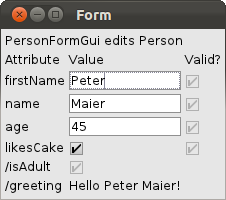
\includegraphics[scale=0.6]{img/form-valid.png}
  \end{columns}
\end{frame}

\begin{frame}
	\frametitle{Case Study} % for adjustments use overpic[grid,tics=10]  
	\begin{overpic}[scale=0.5]%
       {img/guidsl.png}
       \only<2>{
        \put(-2.5,-3){\includegraphics[scale=0.5]%
		{img/guidsl-errors.png}}}
     \end{overpic}
\end{frame}